\documentclass[10pt,a4paper]{article}
\usepackage[margin=0pt]{geometry}
\usepackage[T1]{fontenc}
\usepackage{helvet}
\renewcommand{\familydefault}{\sfdefault}
\usepackage{graphicx,xcolor,tikz}
\pagestyle{empty}
\definecolor{navy}{HTML}{123347}
\definecolor{teal}{HTML}{167D8D}
\definecolor{muted}{HTML}{475866}
\definecolor{pale}{HTML}{8ED8DD}
\definecolor{rulecolour}{HTML}{D4E0E6}
% Positions are PDF points measured from the top-left of A4.
% Edit the text directly; keep the figure in the assets folder.
\newcommand{\block}[5]{\node[anchor=north west,inner sep=0pt,text width=#3pt,text=#4,font=\fontsize{#5}{\dimexpr#5pt*14/10\relax}\selectfont,align=left] at (#1,-#2)}
\newcommand{\classification}{RESEARCH DEMONSTRATION | NOT FOR OPERATIONAL USE}
\begin{document}
\null
\begin{tikzpicture}[remember picture,overlay,x=1pt,y=1pt]
\begin{scope}[shift={(current page.north west)}]
\fill[navy] (0,0) rectangle (595.28,-104);
\node[anchor=north,inner sep=0pt,text=red!65!white,font=\fontsize{8}{10}\selectfont] at (297.64,-7) {\textbf{\classification}};
\block{36}{29}{523}{pale}{10}{\textbf{AAD PLACEMENT / PRODUCT DEVELOPMENT}};
\block{36}{49}{523}{white}{22}{\textbf{Antarctic Fast Ice Watch}};
\block{36}{126}{523}{navy}{15}{Primary and additional observation products};
\block{36}{158}{523}{muted}{10.5}{A weekly one-page bulletin for the Casey, Davis and Mawson approaches. The primary product will be Sentinel-1 fast-ice extent and change maps, updated with suitable overlapping acquisitions (target approximately every four days, subject to coverage and quality). The additional product will be SWOT freeboard maps; thickness estimation will be investigated through validation and explicit uncertainty assessment.};
\block{36}{249}{523}{teal}{10}{\textbf{PRIMARY PRODUCT | FAST-ICE EXTENT AND CHANGE MAPS}};
\node[anchor=north west,inner sep=0pt] at (36,-273) {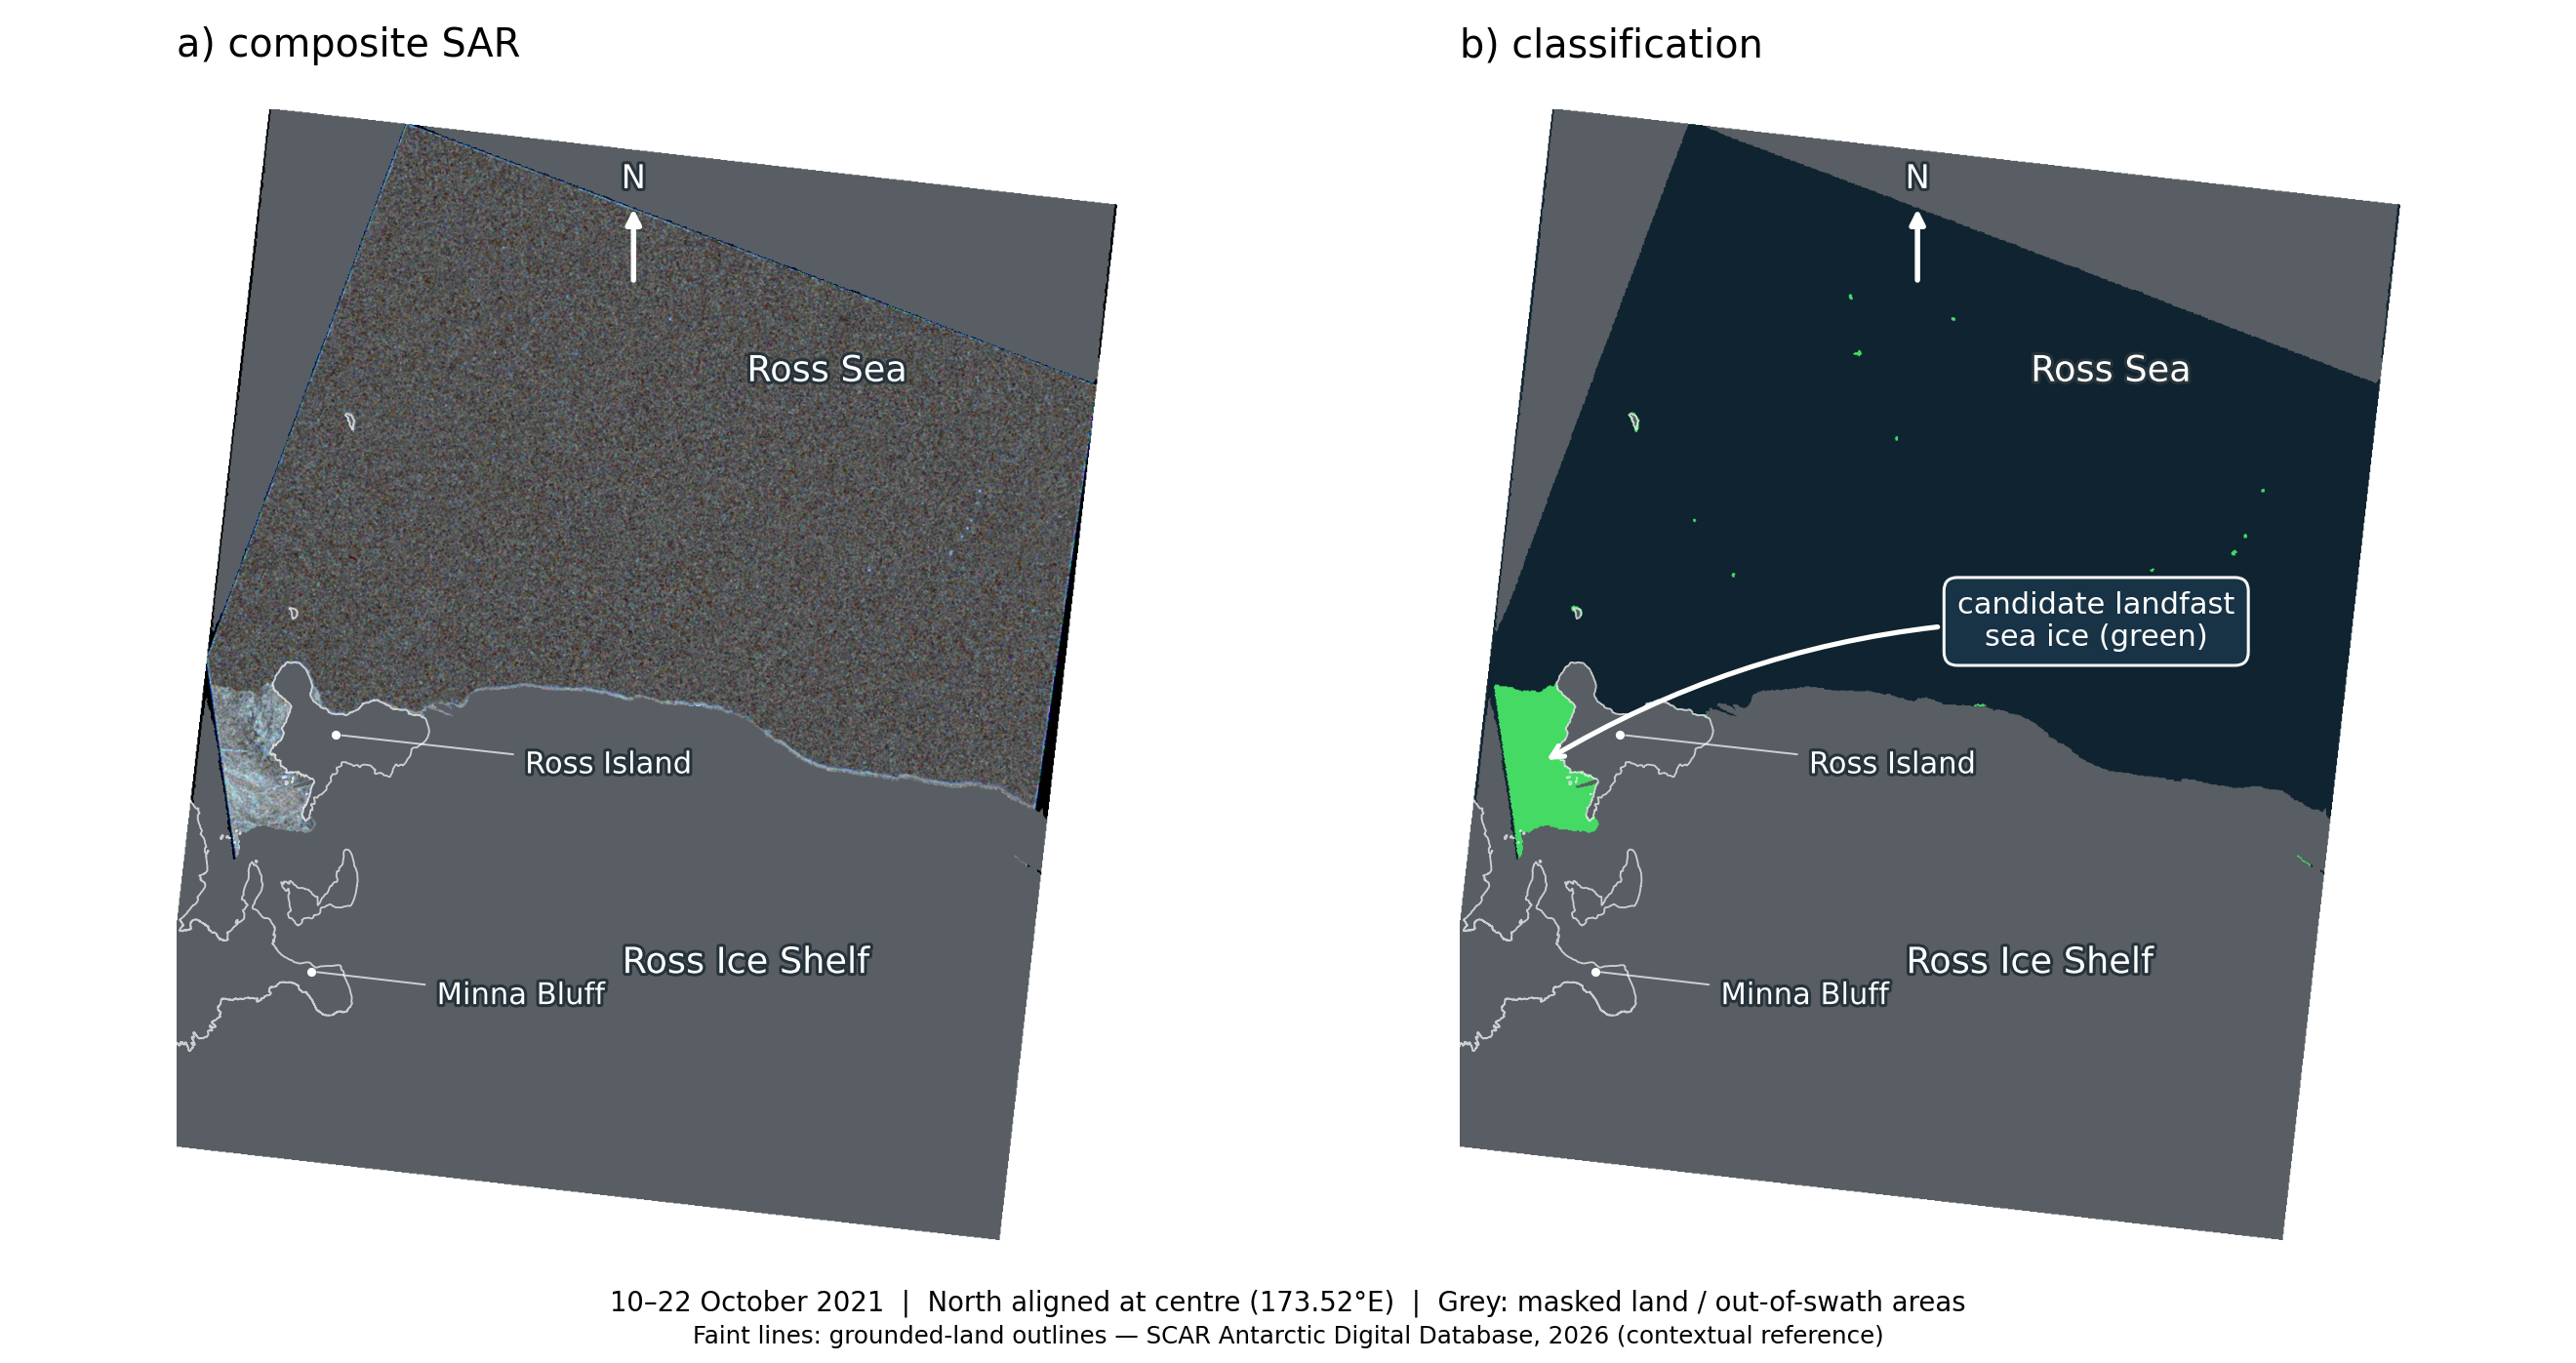
\includegraphics[width=523pt]{assets/fastice_texture_and_segmentation.png}};
\block{36}{553}{523}{muted}{9}{\textbf{Research workflow example:} SAR texture composite and predicted classification, 10--22 October 2021, McMurdo/Ross Sea. Green: candidate landfast sea ice (class 2; originally blue). Grey: masked land/ice shelf and out-of-swath areas. Faint lines: grounded-land outlines from SCAR Antarctic Digital Database, 2026, provided as geographic context. Both panels share orientation and crop. This extent example does not show change.};
\block{36}{611}{523}{teal}{10}{\textbf{ADDITIONAL PRODUCT | SWOT FREEBOARD MAPS}};
\node[anchor=north west,inner sep=0pt] at (36,-635) {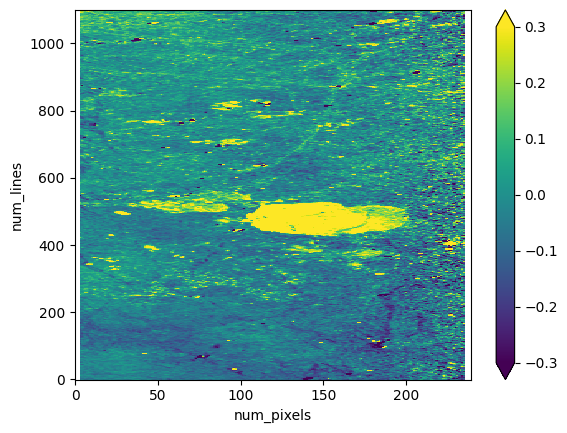
\includegraphics[width=200pt]{assets/alex_swot_research_example.png}};
\block{255}{637}{304}{muted}{9}{\textbf{Research example:} Alex Fraser's Ross Sea demonstration, SWOT cycle 056 / pass 142, acquired 15 September 2026. The notebook plots sea-surface-height anomaly (\texttt{ssha\_karin\_2}, metres), with a quadratic cross-track profile removed. Axes are pixel/line indices; range -0.3 to +0.3 m. This demonstrates relative elevation, not validated freeboard or thickness. The planned additional product requires rigorous retrieval, quality control and uncertainty assessment.};
\draw[rulecolour] (36,-800) -- (559,-800);
\node[anchor=north,inner sep=0pt,text=red,font=\fontsize{8}{10}\selectfont] at (297.64,-808) {\textbf{\classification}};
\end{scope}
\end{tikzpicture}
\end{document}
